\chapter{Szenario}
Im Landwirtschaftsbetrieb in Fuchshain wird ein Kühlsystem verwendet, um die Milch auf die richtige Temperatur zu kühlen. Dabei gelangt die gewonnene Milch in einen Milchtank, welche dann herunter gekühlt wird. In den eigentlichen Kühlvorgang kann nicht eingegriffen werden, weswegen die Vorkühlung der Milch vor dem Milchtank durch den Eiswasserspeicher realisiert werden muss. Dieser Eiswasserspeicher soll durch eine vorhandene PV Anlage gespeist werden.\\
Während der Produktion muss die Milch von 35 auf 4 Grad Celsius abgekühlt werden. Diese Kühlmaßname ist energieaufwändig (304342,5 kJ bei 2500 Liter Milch) \cite{kusow}. Damit die Hauptkühlung entlastet werden kann, soll die Effizienz einer Vorkühlung durch einen Eiswasserspeicher ermittelt werden. Dieser Speicher würde eine Abflachung der Lastspitzen ermöglichen und somit dem Betrieb Geld einsparen. Da die Anschaffung eines Eiswasserspeichers kostspielig ist, soll vorerst durch eine Simulation die Rentabilität ermittelt werden. Dabei wird angenommen, dass eine Vorkühlung der Milch von 35 auf 17 Grad Celsius stattfindet.

\section{Eiswasserspeicher}
Der Eiswasserspeicher kann 164 kg Eis speichern. Er verfügt weiterhin über einen Kompressor der Marke Maneurop MT-22 mit 3,51 kW Leistung. Der Kompressor ist für die Erzeugung des Eises verantwortlich. Weiterhin befindet sich im Speicher die horzontale Kreiselpumpe CEA 70/3/A-V der Firma LOWARA. Die Ladezeit für eine komplette Beladung mit Eis wird mit sechs Stunden angegeben \cite{kusow}.\\
Abbildung \ref{verbrauch1feb} zeigt den Verbrauch der Anlage am 1. Februar 2015 ohne den Betrieb eines Eiswasserspeichers. Die zwei hohen Ausschläge geben die Leistung der zwei Kühlanlagen wieder. Diese Last soll durch einen Eiswasserspeicher gemindert werden, indem eine Vorkühlung stattfindet. In Kombination mit der PV Anlage erzeugt der Eiswasserspeicher einen Energiegehalt zum Vorkühlen, welche die eigentliche Last der Hauptkühlung mindern soll.
 \begin{figure}[H]
 	\centering
 	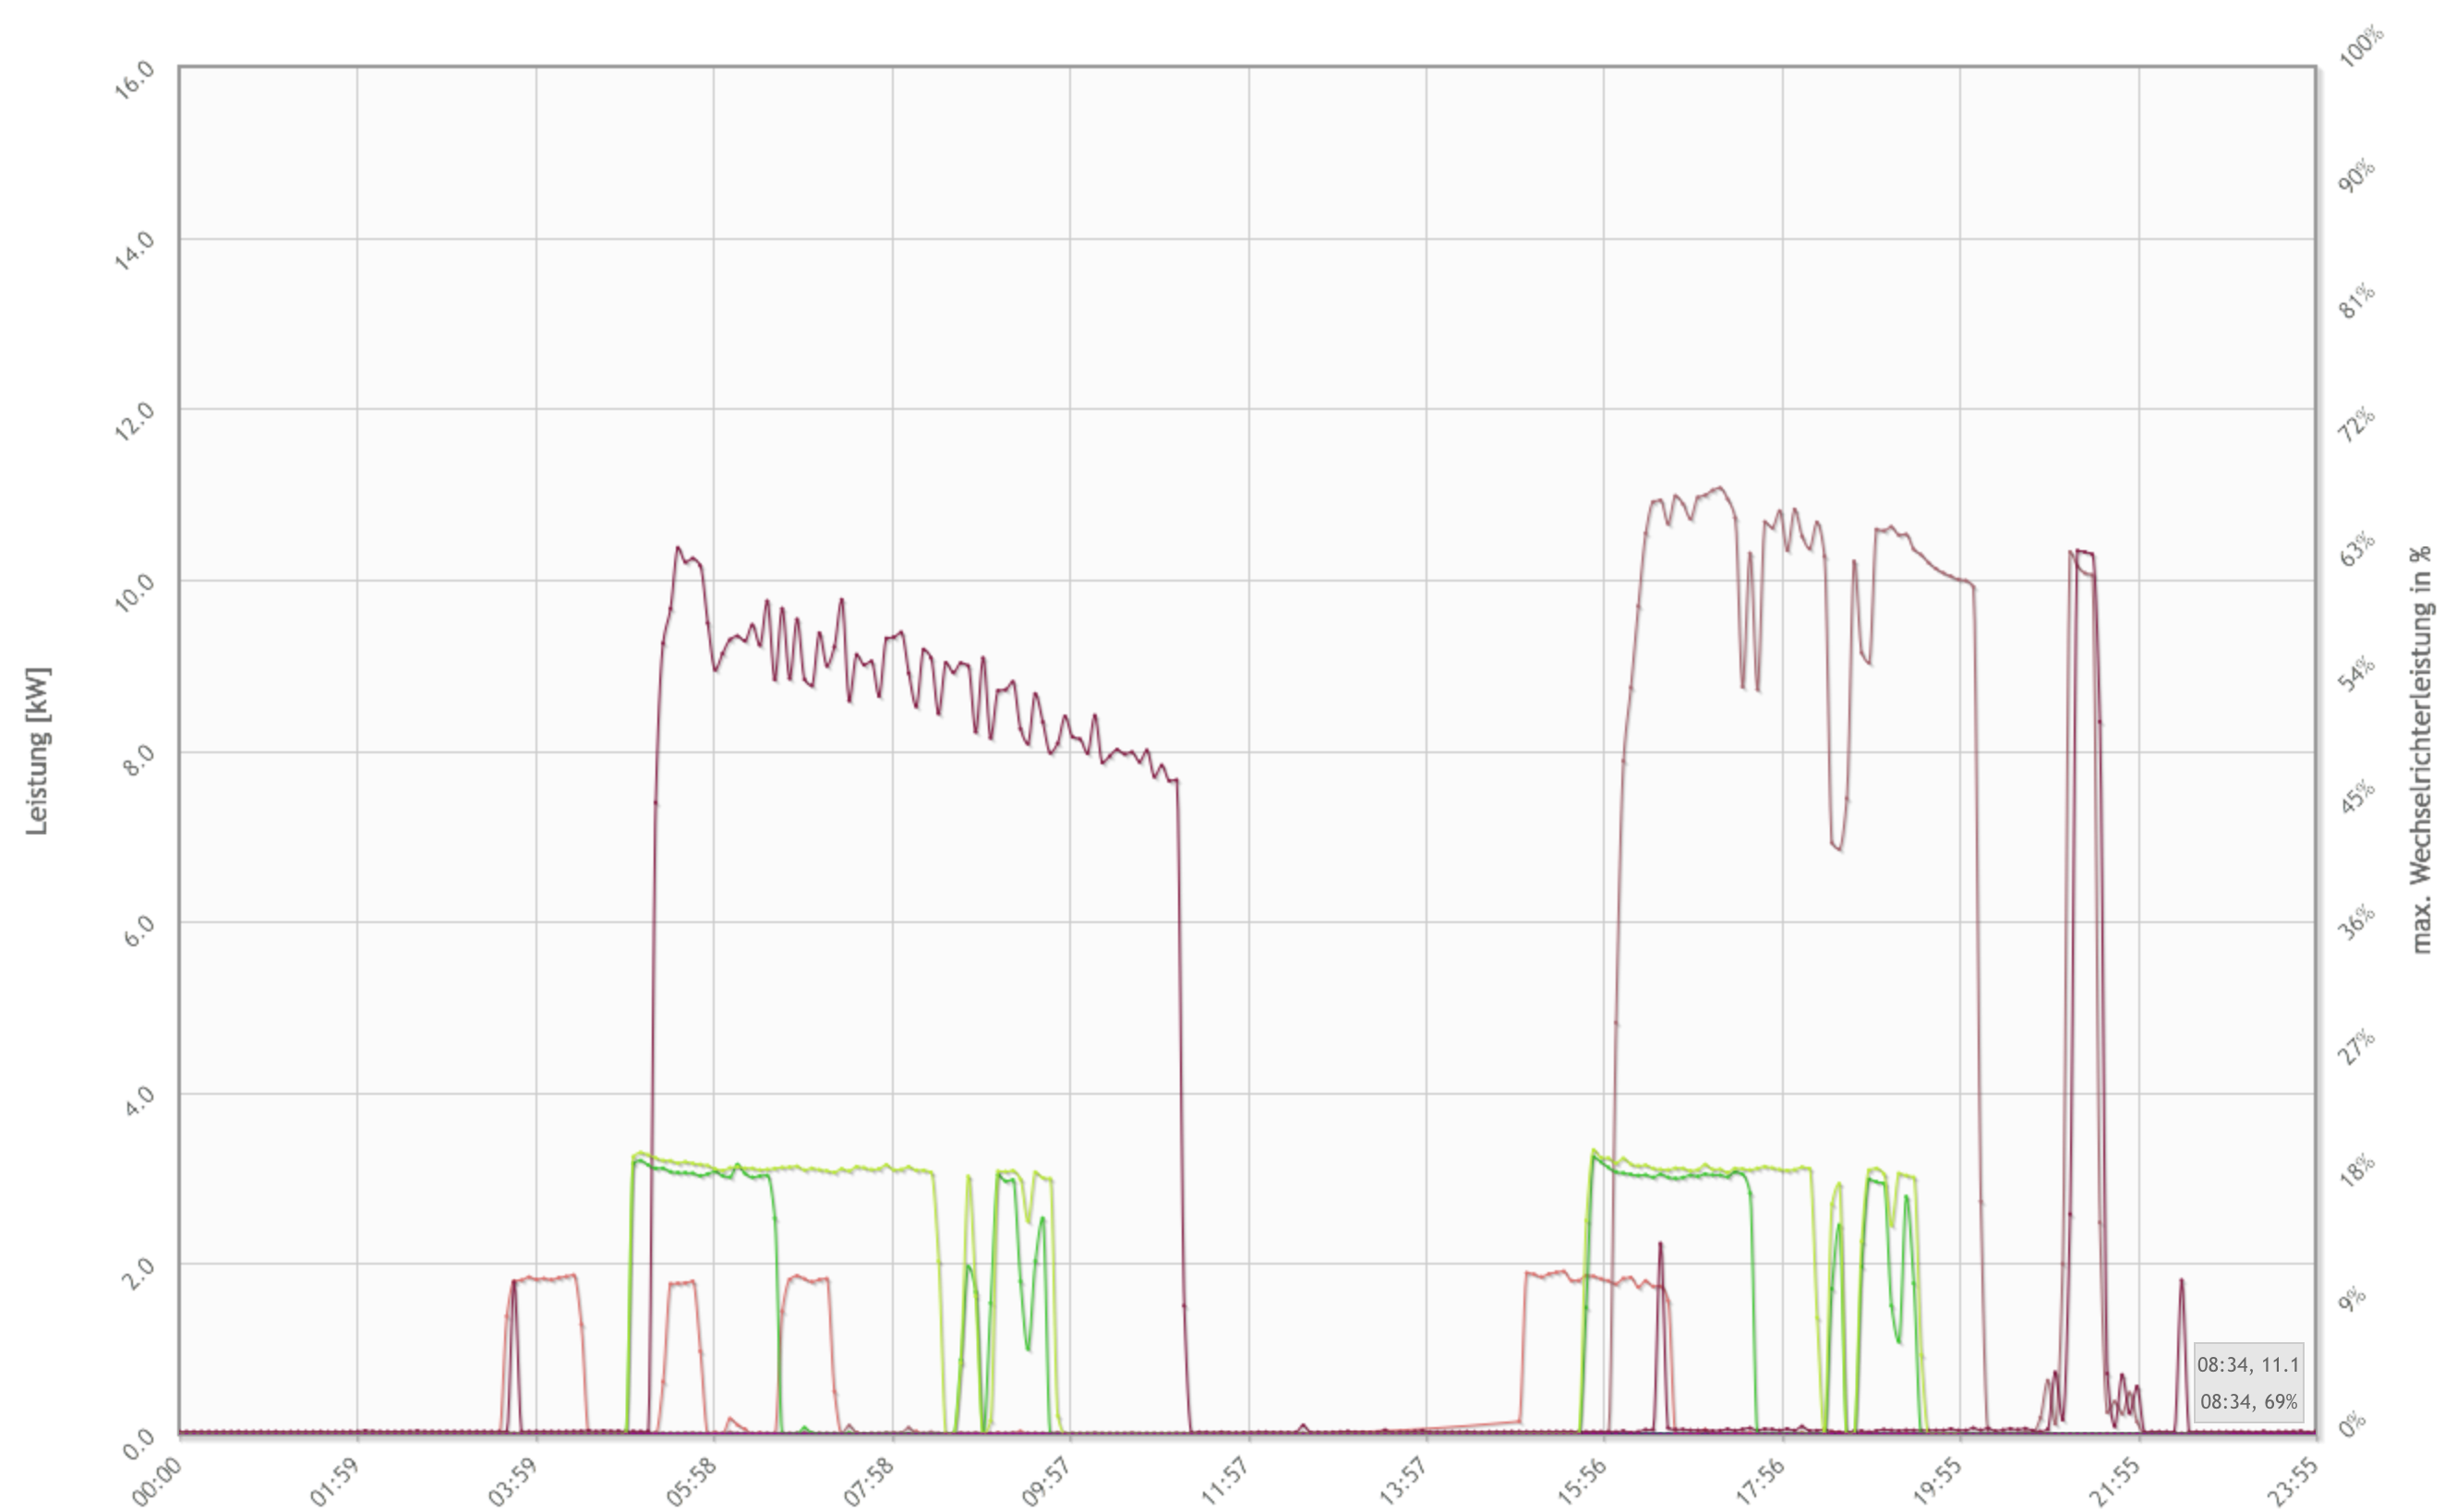
\includegraphics[width=\textwidth]{bilder/verbrauch1feb.png}
 	\caption{Verbrauch 1. Februar 2015}
 	\label{verbrauch1feb}
 \end{figure}

\section{Lösung}\label{solution}
Für die Realisierung des Simulators wurde ein Raspberry PI zur Verfügung gestellt. Dieser soll softwareseitig alle 15 Minuten einen Simulationsschritt durchführen. In einem Schritt wird festgestellt, ob der Speicher beladen bzw. entladen wird. Während den Schritten wird die verrichtete elektrische Arbeit anhand einer S0-Schnittstelle übertragen. Die Leistung für den Ent- und Beladevorgang wurden vorgegeben und sind als konstant anzusehen.\\
Die S0-Schnittstelle ist nach DIN EN 62053-31 spezifiziert und dient zur Übertragung von Verbrauchsmesswerten. Häufiger Einsatz ist die Gebäudeautomatisierung und findet in einer Vielzahl von Messgeräten Anwendung. Elektrische Impulse dienen als Maßeinheit für den Verbrauch eines Geräts. Diese Impulse müssen ein gewisses Muster aufweisen, damit sie als gültiger Impuls gewertet werden. Ein Impuls besteht aus einem \emph{HIGH} und einem \emph{LOW} Signal. HIGH muss ebenso wie LOW mindestens 30 Millisekunden lang sein und die auf bzw. absteigende Flanke muss kleiner als fünf Millisekunden sein. Weiterhin entsprechen in diesem Projekt 1000 Impulse einer verrichteten elektrischen Arbeit von 1000 Wattstunden.